\chapter{Background}
\label{ch:Background}
\section{Quantum Interference (unfinished)}
\label{sec:HOM}
Quantum interference is really important. In fact, a large part of the
verification chapter is concerned with establishing that it's happening. There
is a neat mathematical description of this phonemenon in terms of permanents (or
determinants) of matrices.

Figure~\ref{fig:HoMWalk} shows a more complicated example of quantum
interference, in the scenario of a continuously-coupled walk. The difference
between the three coincidence plots (b-d) will be really important in
chapter~\ref{ch:QCV}.

\begin{figure}
  \centering
  \includegraphics{figures/simplehom.pdf}
  \caption[Quantum interference on a beamsplitter]
  {Quantum interference on a beamsplitter. Two particles are incident on a
  \(50:50\) beamsplitter, one in each of the modes A and B. There are 3 possible
  outcomes at modes A\(^{\prime}\) and B\(^{\prime}\): (a) one particle in each,
  (b) two particles in A\(^{\prime}\), (c) two particles in B\(^{\prime}\). In
  the case of classical (distinguishable) particles, (a) occurs with probability
  0.5 and (b) and (c) occur with probability 0.25. For bosons, the two ways of
  achieving (a) interfere destructively, resulting in an equal superposition of
  (b) and (c). For fermions, the effect of interference (Pauli exclusion) is
  that (b) and (c) are forbidden and (a) is the only possible outcome.}
  \label{fig:SimpleHoM}
\end{figure}

\begin{figure}
  \centering
  \includegraphics{figures/homwalk.pdf}
  \caption[Quantum interference in a continuously-coupled walk]
  {Quantum interference in a 16-mode continously-coupled walk. (a) A single
  photon (bright light) is injected in mode 7, the height of the bar indicates
  the probability of detection at each of the output modes. (b-d) Two particles
  are injected into modes 7 and 8, the intensity of the colour indicates the
  probability of coincident detection at modes \(i\) (horizontal axis) and \(j\)
  (vertical axis) for bosons (b), fermions (d) and distinguishable particles
  (c). The diagonal line indicates `bunched' events where \(i=j\).}
  \label{fig:HoMWalk}
\end{figure}

\section{Evolution of Quantum States}
\label{sec:Evolution}
A large part of quantum mechanics (arguably all of quantum mechanics) concerns
calculating the evolution of quantum systems. At any time, a system in a pure
state\footnote{Except when explicitly stated, I am describing photonic states as
pure.} can be completely described by
its wavefunction, \(\ket{\Psi}\) \cite{pbr}. In the non-relativistic
picture\footnote{I am restricting the discussion to non-relativistic quantum
mechanics, since it offers a valid description of the behaviour of photons,
perhaps surprisingly since they travel at the speed of light.} this
wavefunction evolves according to the Schr\"odinger equation, in terms of the
Hamiltonian, \(\op{H}\):
\begin{equation}
  \op{H} \ket{\Psi} = i \hbar \frac{\partial}{\partial t} \ket{\Psi}
\end{equation}
In the case of a Hamiltonian that is constant in time, we can integrate this
equation to obtain a time-evolution operator (sometimes referred to as a
propagator):
\begin{equation}
  \label{eq:expiht}
  \op{U} \of{t} = e^{-\frac{i}{\hbar} \op{H} t}
\end{equation}
This operator relates a known state of the system at time \(t_{0}\) to the state
of the system at a later (or earlier) time, \(t\), via
\begin{equation}
  \ket{ \Psi \of{t} } = \op{U} \of{t-t_{0}} \ket{ \Psi \of{t_{0}} }
\end{equation}
Another simple case to consider is when the Hamiltonian varies but is piecewise
constant in time. In this case each constant segment has its own time evolution
operator, \(\op{U}_{i}\) and  the overall time evolution operator is just the
(appropriately ordered) product of these:
\begin{equation}
  \op{U} = \op{U}_{n} \cdot \op{U}_{n-1} \dots \op{U}_{2} \cdot \op{U}_{1}
\end{equation}
When the Hamiltonian is Hermitian, which it must be for a closed quantum system
(in order to conserve energy), the time evolution operator is unitary.

In the case of photonics (or at least the cases that I will discuss in this
thesis), the state space is discrete and finite, meaning that the wavefunction
can be expressed exactly as a complex vector of unit magnitude. The number of
dimensions required is the number of optical modes, be they spatial,
polarisation or some other degree of freedom. The Hamiltonians that we consider
are piecewise constant in time (e.g. the application of a waveplate in bulk or
a directional coupler in integrated optics\footnote{between these optical
components, the Hamiltonian is diagonal with uniform elements.}) so the time
evolution operator is a natural description.

When considering Hamiltonians on a discrete (\(m\)-dimensional) space, for
example in the case of an \(m\) mode quantum walk \cite{walks-peruzzo}, the
matrix exponential in equation~\ref{eq:expiht} can be performed classically in
time polynomial in \(m\). This observation, along with the ability to realise
any unitary operator in linear optics (see section~\ref{sec:ReckScheme}), is the
basis of the quantum simulations performed in chapter~\ref{ch:Simulations}.

This model can be extended to consider non-Hermitian Hamiltonians, in which
case the same mathematics applies, but equation~\ref{eq:expiht} results in a 
non-unitary operator. Physically, we associate this with an open quantum system,
or a system coupled to some external degrees of freedom (an environment).
Chapter~\ref{ch:Simulations} also describes quantum simulations of this kind of
coupled system.

\section{A universal circuit for linear optics}
\label{sec:ReckScheme}
\begin{figure}[p]
  \begin{subfigure}{\textwidth}
    \centering
    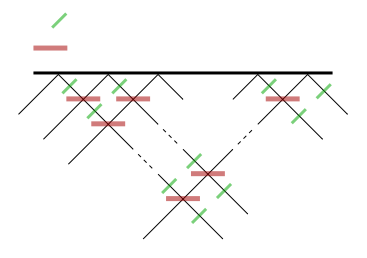
\includegraphics{figures/reck_original}
    \caption{The original Reck scheme, implemented in bulk optics. As with all
    circuits in bulk optics, achieving phase stability in this system would be
    very difficult.}
    \label{fig:ReckOriginal}
  \end{subfigure} \\
  \vspace{1cm} \\
  \begin{subfigure}{\textwidth}
    \centering
    \includegraphics{figures/reck_general}
    \caption{A more modern take on the Reck scheme. Here we envisage using
    a triangular array of
    Mach-Zehnder interferometers (MZIs) on an integrated platform, thus solving
    the phase stability problem.}
    \label{fig:ReckGeneral}
  \end{subfigure}
  \caption[The Reck scheme, in both its original conception and an integrated
  optics version]{The Reck scheme, in both its original conception and an
  integrated
  optics version. In both systems, light enters from the left and the device
  performs a unitary transformation on the modes. Variable-reflectivity
  beamsplitters and variable phase shifts are needed in order to make the
  circuit's operation reconfigurable to any unitary transformation. In the
  bulk scheme, I have omitted any specifics, but in the integrated version these
  could be implemented with directional couplers and thermal or electro-optic
  phase shifts \cite{peteschip}.}
  \label{fig:ReckScheme}
\end{figure}
Any lossless\footnote{In practical devices, this approximation is very good.
(about 1dB/cm in silica devices)} linear optical device can be
described by a unitary matrix operating on the optical modes. A device with
\(m\) input and \(m\) output modes will be described by an \(m \by m\) unitary.
In~\cite{reck}, it is shown that the converse is true: any unitary matrix can
be realised by a linear optical circuit. A constructive proof of this is
presented, and an architecture for a `universal circuit' is proposed (see
figure~\ref{fig:ReckOriginal}). Universal in this context refers to a linear
optical circuit with adjustable components (beamsplitters with variable
reflectivity and variable phase shifts), which can be configured into any
unitary.

This result has profound consequences for experimental quantum photonics.
It implies that when such a circuit is built, \emph{all} other linear optical
devices will become redundant, being just specific configurations of the
general circuit. Rapid progress in fabrication and control of integrated optics
has recently brought a \(6 \by 6\) reconfigurable circuit to the lab, and some
of the data in chapter~\ref{ch:Simulations} were taken on this device.

\section{Boson Sampling}
\label{sec:BosonSampling}
\begin{figure}
  \includegraphics{figures/bosonsampling}
  \caption[BosonSampling in linear optics]
  {(a) \bosonsampling{} in linear optics. \(p\) photons are injected into the
  first \(p\) inputs of an \(m\) mode linear optical circuit, then detected at
  the output, post-selecting on all photons occupying distinct modes. The
  probability of this event occurring depends on the description of the circuit,
  a unitary matrix \(\mat{U}\) (b). It can be calculated by taking columns of
  the unitary corresponding to the input modes (shaded red) and rows
  corresponding to the detector clicks (shaded green), the intersection of which
  defines a \(p \by p\) submatrix (c). The probability of the detection event is
  given by the absolute square of the permanent of this submatrix.}
  \label{fig:BosonSampling}
\end{figure}
This section presents a brief review of \bosonsampling{}: a sampling algorithm
presented by Aaronson and Arkhipov in~\cite{bosonsampling} (AA). None of
development or complexity analysis of this algorithm is my own work, but it
provides useful context for material in chapter~\ref{ch:DirectDialling} and
section~\ref{sec:RStar}.

In their development of the \bosonsampling{} problem, AA have described a
computational task that can be performed by a linear optical network which we
strongly believe cannot be performed by a classical computer. If we find no
fundamental obstacle to demonstrating \bosonsampling{} in practice (or even
better, actually do it!), this would force us to abandon (or at least further
extentd) the Extendend Church-Turing Thesis (ECT). First though, we need to
better understand this \emph{strong belief} on which the result is based.

The nature of the proof is that, if
the exact form of the \bosonsampling{} problem were performed classically, it
would imply the collapse of the polynomial hierarchy. While this is not
expressly forbidden by complexity theory, the same can be said about the
conservation of energy. The implications to a complexity theorist are equally
absurd. The caveat to this proof is that even the quantum computer does not
perform \bosonsampling{} exactly, so this is an unfair demand to place on a
classical competitor. In the case of a reasonable approximation, two unproved
but plausible conjectures (backed up by numerical evidence) are required to
imply the same collapse of the polynomial hierarchy.

Against the better known challenger to the ECT, using Shor's algorithm to factor
large numbers, this actually compares very favourably. If somebody were to
announce tomorrow that they had developed a classical algorithm that could
factor numbers in polynomial time, the news would be very disruptive to
everyday life (and quantum computing research budgets) but it wouldn't have a
profound effect on complexity theory. A single decision problem (factoring)
would have to be moved from NP to P. We already know that factoring is not
NP-complete, so it wouldn't even have any implications on the long-standing
question of whether P=NP.

I will now briefly describe practical \bosonsampling{}, before returning to
consider how valuable it is as a computational model. As the name suggests, a
demonstration of \bosonsampling{} involves taking samples from a probability
distribution, in this case corresponding to the probabilities of detection
events in a linear optics experiment as shown in figure~\ref{fig:BosonSampling}.
The linear optics circuit on \(m\) modes is described by an \(m \by m\) unitary
matrix, \(\mat{U}\). We inject \(p\) photons into the first \(p\) input modes
and detect on all output modes. There are \(\comb{m+p-1}{p}\) possible output
configurations, of which \(\comb{m}{p}\) occupy the \emph{collision-free
subspace} i.e.\ where no mode contains more than one photon.

In order to calculate the probability of any detection event, we take the
indices of occupied input modes, \(\left\{ s_{0}, s_{1}, \dots, s_{p-1} \right\}
\) (usually assumed to be \(0, 1, \dots p-1\) without loss of generality) and
the indices of occupied output modes, \(\left\{ t_{0}, t_{1}, \dots, t_{p-1}
\right\}\). From the unitary \(\mat{U}\), we select rows corresponding to the
output modes and columns corresponding to the input modes, and take the
submatrix \(\mat{U}_{ST}\) defined by their intersections. The probability of
the event is the absolute square of the permanent of this submatrix, \(\abs{
\perm \of{ \mat{U}_{ST} }} \). This process is illustrated in
figure~\ref{fig:BosonSampling}.

This description gives us some intuition into why it may be hard to perform
\bosonsampling{} classically. The size of the distribution---\( \comb{m+p-1}{p}
\)---increases combinatorially with the number of photons\footnote{Provided that
the number of modes also increases accordingly}, so the memory requirement for
storing the entire distribution is not polynomial in \(p\). Further, even if one
didn't have to store the entire distribution to perform a sampling (and we
wouldn't expect to have to do this), just computing one element of it requires
evaluation of the permanent of a \(p \by p\) complex matrix. Computing
permanents exactly is \# P complete \cite{valiant} and the fastest known
algorithm (Ryser's algorithm) has running time \(\bigo \of{ p 2^{p} }\). This is
by no means a proof that \bosonsampling{} is classically hard (if we inject
classical, distinguishable particles, we can sample the output distribution
without explicitly calculating \emph{any} \(p\)-photon probabilities), but it
does strongly suggest a link between \bosonsampling{} and the evaluation of
permanents.

Now one may ask how this is considered a computation at all.
After all, it does not result in any deterministic outcome. A plausible
complaint might be that just because something cannot be modeled classically,
it doesn't make it a classically intractable computation. We can illustrate
this by pointing to a cow, and using it to define the \alg{Cow} algorithm.
After all, it is beyond the powers of our classical computers to model such a
large ensemble of atoms. Therefore does \alg{Cow} not disprove the
Church-Turing thesis?

The response requires us to look at the other feature of computations: the
input. We have no control over the input to \alg{Cow}, and even if we did it
would require a very large number of parameters (surely exponential in the size
of the cow?). On the other hand \bosonsampling{} is controlled by a small number
of input parameters (\(\bigo \of{m^{2}}\) for an \(m\) mode linear optical
circuit) and we have direct control over all of them.

A final important discussion surrounding \bosonsampling{} is that of
verification: if we have a large Boson Sampler, how can we confirm that it is
operating correctly? There is an important distinction to be made here between
a quantum algorithm like Shor factoring, which is in NP and \bosonsampling{},
which is not. In the former case, the problem satisfies the \emph{short
certificate} property, guaranteeing that the output of any task in NP can be
verified by in classical polynomial time. A valid certificate in the case of
factoring is the prime factors, since these can be efficiently multiplied
together to verify correct operation. Tasks outside NP have no such guarantee.
This difficulty was raised in the original proposal by Aaronson and Arkhipov,
and highlighted again by Gogolin et al \cite{gogolin}, who showed that under
certain circumstances it would be information-theoretically impossible to
distinguish the output of a Boson Sampler from that of a uniform sampling of the
configuration space. In chapter~\ref{ch:QCV} I describe methods to address this
problem, and gain some confidence in the correct operation of a \bosonsampling{}
device.
